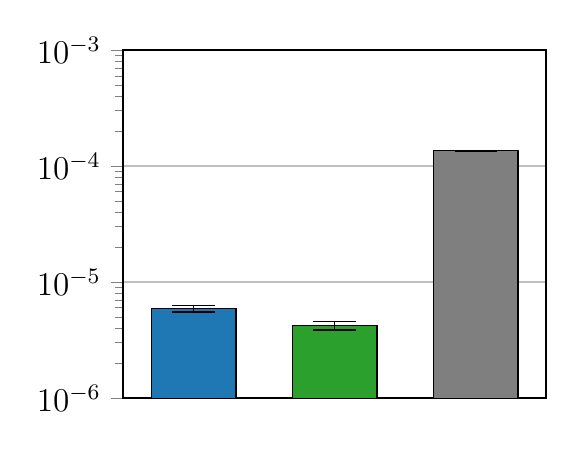
\begin{tikzpicture}
\definecolor{darkgray}{RGB}{169,169,169}
\definecolor{darkorange25512714}{RGB}{255,127,14}
\definecolor{darkslategray38}{RGB}{38,38,38}
\definecolor{darkturquoise23190207}{RGB}{23,190,207}
\definecolor{gray127}{RGB}{127,127,127}
\definecolor{lightgray204}{RGB}{204,204,204}
\definecolor{mediumpurple148103189}{RGB}{148,103,189}
\definecolor{orchid227119194}{RGB}{227,119,194}
\definecolor{sienna1408675}{RGB}{140,86,75}
\definecolor{steelblue31119180}{RGB}{31,119,180}
\definecolor{steelblue76114176}{RGB}{76,114,176}
\definecolor{tabgreen}{RGB}{44,160,44}

\begin{semilogyaxis}[
  line width=0.8pt,
  axis line style={black},
  xmin=-0.5, xmax=2.5,
  xtick=\empty,
  ymin=1e-6, ymax=1e-3,
  ymajorgrids,
  height=6cm,
  ytick pos=left,
  % width=7cm,
  % x grid style={lightgray204},
  % y grid style={lightgray204},
  % axis line style={darkgray},
  tick align=outside,
  % ylabel={Full Rollout MSE},
  ylabel style={font=\LARGE},
  tick label style={font=\large},
]

% Bars (bottom anchored at ymin=1e-7)
% 0: pointpatch (tab:blue)
\draw[fill=steelblue31119180, draw=black, line width=0.5pt] (axis cs:-0.3, 1e-7) rectangle (axis cs:0.3, 0.00000590559102420229);
% 1: oracle (tab:green)
\draw[fill=tabgreen, draw=black, line width=0.5pt] (axis cs:0.7, 1e-7) rectangle (axis cs:1.3, 0.00000421955195406554);
% 3: dummy (tab:gray)
\draw[fill=gray127, draw=black, line width=0.5pt] (axis cs:1.7, 1e-7) rectangle (axis cs:2.3, 0.000135723821585998);

% Error bars
% 0: pointpatch
\draw[black, semithick] (axis cs:0, 0.00000553021868654469
) -- (axis cs:0, 0.0000062809633618599);
\draw[black, semithick] (axis cs:-0.15, 0.00000553021868654469) -- (axis cs:0.15, 0.00000553021868654469);
\draw[black, semithick] (axis cs:-0.15, 0.0000062809633618599) -- (axis cs:0.15, 0.0000062809633618599);
% 1: oracle
\draw[black, semithick] (axis cs:1, 0.00000387946136015671) -- (axis cs:1, 0.00000455964254797436);
\draw[black, semithick] (axis cs:0.85, 0.00000387946136015671) -- (axis cs:1.15, 0.00000387946136015671);
\draw[black, semithick] (axis cs:0.85, 0.00000455964254797436) -- (axis cs:1.15, 0.00000455964254797436);
% 3: dummy
\draw[black, semithick] (axis cs:2, 0.000135091322590597) -- (axis cs:2, 0.000136356320581399);
\draw[black, semithick] (axis cs:1.85, 0.000135091322590597) -- (axis cs:2.15, 0.000135091322590597);
\draw[black, semithick] (axis cs:1.85, 0.000136356320581399) -- (axis cs:2.15, 0.000136356320581399);


\end{semilogyaxis}
\end{tikzpicture}